% !TeX root = ../main.tex


\section{8 chapter}
Power/influence and contingency theories of leadership

\subsection{Power and Influence Concepts} % (fold)
\label{sub:power_and_influence_concepts}

\begin{itemize}
	\item power is the capacity of one party (the agent) to influence another party (the target).
	\begin{itemize}
		\item the agent can be group or organization
		\item  power is a dynamic variable that changes ac conditions change
	\end{itemize}
	

	\item authority: the right to make particular types of decisions for the organization
	\begin{itemize}
		\item also involves the right to control over things such as money, resources, equipment, and materials
		\item scope of authority is the range of requests and actions that can be made and taken.
	\end{itemize}

	\item 3 influence processes
	\begin{itemize}
		\item instrumental compliance ­ the target person carries out a requested action for the purpose of obtaining a tangible reward or avoiding a punishment
		\item internalization ­ the target person becomes committed to support and implement proposals espoused by the agent because they appear intrinsically desirable and correct
		\item personal identification ­ the target person imitates the agent’s behavior or adopts the same attitudes to please the agent and to be like the agent
	\end{itemize}

	\item outcomes of influence attempts
	\begin{itemize}
		\item commitment ­the target person agrees with a decision or request from the agent and makes a great effort to carry out the request or implement the decision effectively
		\item compliance ­the target is willing to do what the agent asks but is apathetic rathern than enthusiastic about it and will make only minimal effort 
		\item resistance ­the target person is opposed to the proposal or request, rather than merely indifferent about it, and actively tries to avoid carrying it out
	\end{itemize}
	
\end{itemize}


% subsection power_and_influence_concepts (end)

\subsection{Power Sources} % (fold)
\label{sub:power_sources}


\begin{itemize}
	\item Position Power
	\begin{itemize}
		\item Legitimate Power - Power stemming from formal authority over work activities . Compliance is more likely for members who identify with the organization and are loyal to it. Acceptance of authority depends on whether the agent is perceived to be a legitimate occupant of his leadership position.
			\begin{itemize}
				\item Make polite, clear requests.
				\item Explain the reasons for a request.
				\item Don’t exceed your scope of authority.
			\end{itemize}
		\item Reward Power - the perception by the target person that an agent controls important resources and rewards desired by the target person. Managers usually have much more reward power over subordinates than over peers or superiors. One form of reward power over subordinates is the authority to give pay increases, bonuses
			\begin{itemize}
				\item Offer the type of rewards that people desire.
				\item Offer rewards that are fair and ethical.
				\item Don’t promise more than you can deliver.
			\end{itemize}
		\item Coercive Power - Authority over punishments. It is best to avoid using coercion except when absolutely necessary, because it is difficult to use and likely to result in undesirable side effects
			\begin{itemize}
				\item Explain rules and requirements, and ensure that people understand the serious consequences of violations.
				\item Respond to infractions promptly and consistently without showing any favoritism to particular individuals.
				\item Investigate to get the facts before using reprimands or punishment, and avoid jumping to conclusions or making hasty accusations.
			\end{itemize}
		\item Information Power - This type of power involves both the access to vital information and control over its distribution to others. Control over information is a source of upward influence as well as downward and lateral influence
		\item Ecological Power (situational engineering) - Control over the physical environment, technology, and organization of the work.
		\end{itemize}
	\item Personal Power
	\begin{itemize}
		\item Referent Power - derived from the desire of others to please an agent toward whom they have strong feelings of affection, admiration, and loyalty. The strongest form of referent power involves the influence process called personal identification
			\begin{itemize}
				\item Show acceptance and positive regard.
				\item Be supportive and helpful.
				\item Use sincere forms of ingratiation
			\end{itemize}
		\item Expert Power - Task-relevant knowledge and skill are a major source of personal power. Dependency is increased when the target person cannot easily find another source of advice besides the agent
			\begin{itemize}
				\item Explain the reasons for a request or proposal and why it is important.
				\item Provide evidence that a proposal will be successful.
				\item Don’t make rash, careless, or inconsistent statements.
			\end{itemize}
	\end{itemize}
\end{itemize}
% subsection power_sources (end)

\subsection{How Power Is Gained or Lost} % (fold)
\label{sub:how_power_is_gained_or_lost}
Power is not a static condition; it changes over time due to changing conditions and the actions of individuals and coalitions

\subsubsection{Social Exchange Theory} % (fold)
\label{ssub:social_exchange_theory}
	In a group, the amount of status and power accorded to an elected or emergent leader by other members depends on the person’s loyalty, demonstrated competence, and contribution to the attainment of shared objectives. Members expectations about what leadership role a person should have in the group are influenced by the person’s loyalty and demonstrated competence. If the leader’s proposal prove to be a failure, then terms of the exchange relationship are likely to be reassessed by the group. A leader who fails to show initiative and deal decisively with serious problems will lose esteem and influence, just as a leader who proposes actions that are unsuccessful.
% subsubsection social_exchange_theory (end)


\subsubsection{strategic contingencies theory} % (fold)
\label{ssub:strategic_contingencies_theory}
	How some organizational subunits gain or lose power to influence important decisions such as determination of the organization’s competitive strategy and the allocation of resources to subunits and activities.
	\\The power of subunits depends on (1) expertise in coping with important problems, (2) centrality of the subunit within the workflow, (3) the extent to which the subunit’s expertise is unique rather than substitutable. The more unique and irreplaceable the expertise required to solve critical problems, the more power is gained from possessing this expertise. Increase expert power can result in increased legitimate power.
% subsubsection strategic_contingencies_theory (end)


\subsubsection{Institutionalization of Power} % (fold)
\label{ssub:institutionalization_of_power}
	The process for using political tactics to increase influence or protect existing power. A powerful subunit can get its members appointed to key leadership positions where they will promote the subunit’s objective.

% subsubsection institutionalization_of_power (end)

% subsection how_power_is_gained_or_lost (end)

\subsection{Proactive Influence Tactics} % (fold)
\label{sub:proactive_influence_tactics}
	proactive influence tactic - behavior used intentionally to gain acceptance of a request or support for a proposal

	\begin{itemize}
		\item Core Tactics  - often successful for influencing target commitment to carry out a request or support a proposal
		\begin{itemize}
			\item Rational Persuasion: The agent uses logical arguments and factual evidence to show a proposal or request is feasible and relevant for attaining important task objectives.
				\begin{itemize}
					\item Explain in detail why a request or proposal is important.
					\item Use facts and logic to make a clear case in support of a request or proposal.
				\end{itemize}
			\item Inspirational Appeals: The agent makes an appeal to values and ideals or seeks to arouse the target person’s emotions to gain commitment for a request or proposal.
				\begin{itemize}
					\item Describe a proposed change as an exciting and worthwhile opportunity.
					\item Link a proposed activity or change to the person’s ideals and values.
				\end{itemize}
			\item Consultation: The agent encourages the target to suggest improvements in a proposal or to help plan an activity or change for which the target person’s support and assistance are desired.
				\begin{itemize}
					\item State your objective, and ask what the person can do to help attain it.
					\item Ask for suggestions on how to improve a tentative proposal.
				\end{itemize}
			\item Collaboration: The agent offers to provide relevant resources and assistance if the target will carry out a request or approve a proposed change.
				\begin{itemize}
					\item Offer to show the person how to perform a requested task.
					\item Offer to provide necessary resources.
				\end{itemize}
		\end{itemize}
		
		\item Other Tactics
		\begin{itemize}
			\item Apprising: The agent explains how carrying out a request or supporting a proposal will benefit the target personally or help advance the target person’s career.
				\begin{itemize}
					\item Explain how the person could benefit from carrying out a requested task.
					\item Explain how the task you want the person to do would help his/her career.
				\end{itemize}
			\item Ingratiation: The agent uses praise and flattery before or during an influence attempt, or expresses confidence in the target’s ability to carry out a difficult request.
				\begin{itemize}
					\item Say that the person has the special skills or knowledge needed to carry out a request.
					\item Praise the person’s past achievements when asking him/her to do another task.
				\end{itemize}
			\item Personal Appeals: The agent asks the target to carry out a request or support a proposal out of friendship, or asks for a personal favor before saying what it is.
				\begin{itemize}
					\item Ask the person to do a favor for you as a friend.
					\item Ask for his /her help as a personal favor.
				\end{itemize}
			\item Exchange: The agent offers an incentive, suggests an exchange of favors, or indicates willingness to reciprocate at a later time if the target will do what the agent requests.
				\begin{itemize}
					\item Offer something the person wants in exchange for providing help on a task or project.
					\item Offer to do a specific task or favor in return for compliance with a request
				\end{itemize}
			\item Coalition Tactics: The agent seeks the aid of others to persuade the target to do something, or uses the support of others as a reason for the target to agree.
				\begin{itemize}
					\item Mention the names of others who endorse a proposal when asking the person to support it.
					\item Get others to explain to the person why they support a proposed activity or change.
				\end{itemize}
			\item Legitimating Tactics: The agent seeks to establish the legitimacy of a request or to verify authority to make it by referring to rules, policies, contracts, or precedent.
				\begin{itemize}
					\item Explain that your request or proposal is consistent with official rules and policies.
					\item Point out that your request or proposal is consistent with a prior agreement or contract.
				\end{itemize}
			\item Pressure: The agent uses demands, threats, frequent checking, or persistent reminders to 	influence the target to carry out a request.
				\begin{itemize}
					\item Keep asking the person in a persistent way to say yes to a request.
					\item Insist in an assertive way that the person must do what you ask.
				\end{itemize}
		\end{itemize}
	\end{itemize}

	\begin{figure}[t]
	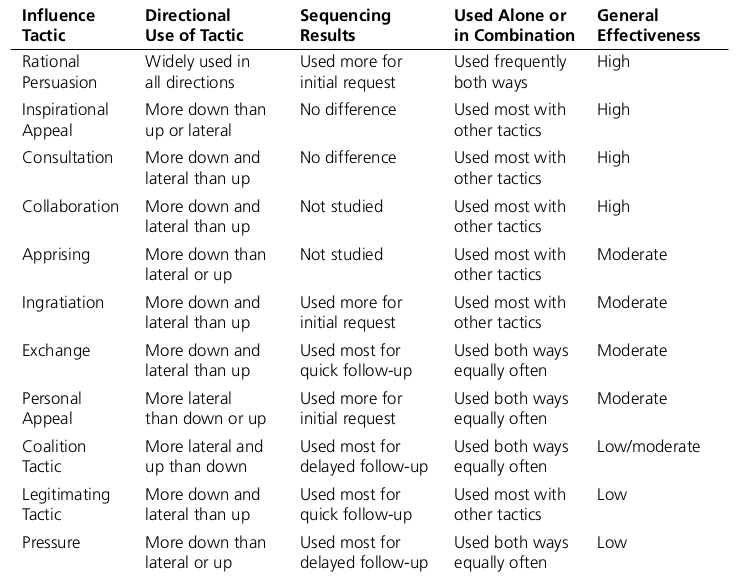
\includegraphics[width=15cm]{proactiveInfluence}
	\centering
	\end{figure}
% subsection proactive_influence_tactics (end)

\subsection{Key Terms} % (fold)
\label{sub:key_terms}
apprising
coercive power
collaboration
commitment
compliance
consultation
ecological power
exchange tactics
expert power
information power
ingratiation
inspirational appeals
institutionalization of power
internalization
legitimate power
legitimating tactic
personal appeal
personal identification
personal power
position power
pressure tactics
proactive influence tactic
rational persuasion
referent power
resistance
reward power
scope of authority

% subsection key_terms (end)